\documentclass[10pt]{article}
\usepackage[margin=0.85in]{geometry}
\usepackage{amsmath,amssymb,amsfonts}
\usepackage{graphicx}
\usepackage{booktabs}
\usepackage{xcolor}
\usepackage{hyperref}
\usepackage{caption}
\hypersetup{colorlinks,linkcolor=blue,urlcolor=blue}

\title{OptB+ with Exact Cube-Cell Mass Integration\\
\large{Replacing vertex step-summation by per-cell Gauss--Legendre integration}}
\author{K=3 dd--qd study, FIXED-POINT-FACTORY}
\date{\today}

\begin{document}
\maketitle

\section{Motivation and construction}

The existing Option B$+$ operator builds the per-slice empirical CDF
$F_v(p\mid u_k)$ by summing trapezoid weights over cube cells whose vertex
$P$-value is below $p$. Concretely, for each slice $k$ it iterates over
the $G^2$ cube vertices $(u_a^{(i)},u_b^{(j)})$ and accumulates
\begin{equation}\label{eq:step}
  \widetilde F_v(p\mid u_k)
  \;=\; \sum_{(i,j)\,:\,P_{k,i,j}\le p}
                w_a^{(i)}\,w_b^{(j)}\,f_v(u_a^{(i)})\,f_v(u_b^{(j)}),
\end{equation}
i.e.\ each cube cell's full Gaussian mass is attributed to a single point at
its $\emph{vertex}$ $P$. The resulting CDF is a step function with $G^2$
knots, on which PCHIP is fitted and the derivative gives the density
$a_v(p,u_k)$, hence
$\mu(p,u_k)=f_1 a_1/(f_0 a_0+f_1 a_1)$.

The dominant error of \eqref{eq:step} is the loss of within-cell sensitivity:
if a single cube cell has its $P$ values varying over a window $\Delta P$,
all of its mass is collapsed to one knot, whereas the true measure spreads
that mass over $\Delta P$. This produces an over-confident CDF, hence the
PCHIP-density misses spikes.

\paragraph{Exact-mass construction.} Within each $(u_a,u_b)$ cell of size
$\Delta u_a\times\Delta u_b$ we use the bilinear interpolant
\begin{equation}
  \widehat P(s,t) \;=\; (1{-}s)(1{-}t)P_{00} + s(1{-}t)P_{10}
                          + (1{-}s)t\,P_{01} + s\,t\,P_{11},
  \qquad (s,t)\in[0,1]^2.
\end{equation}
The true cell contribution to $F_v(p\mid u_k)$ at fixed $u_k$ is
\begin{equation}\label{eq:cell-int}
  F_v^{\rm cell}(p)
  = \Delta u_a\Delta u_b \int\!\!\!\!\int_{[0,1]^2}
       \mathbf 1\{\widehat P(s,t)\le p\}\,
       f_v\bigl(u_a(s)\bigr)\,f_v\bigl(u_b(t)\bigr)\,ds\,dt.
\end{equation}
Rather than computing the level set $\{\widehat P\le p\}$ analytically (it
is a region bounded by a hyperbola), we replace the inner double-integral
by a tensor Gauss--Legendre rule of $\text{NQK}\times\text{NQK}$ nodes,
yielding $\text{NQK}^2$ \emph{micro-cell} contributions per cube cell. Each
micro-cell is a triplet
$(\widehat P(s_q,t_r),\ w_v^{(qr)})$ with weight
\[
  w_v^{(qr)} \;=\; w_q^{\rm GL}\,w_r^{\rm GL}\,
                       \Delta u_a\Delta u_b\,f_v(u_a(s_q))\,f_v(u_b(t_r)).
\]
We then sort all $(G-1)^2\cdot\text{NQK}^2$ micro-cells per slice by
$\widehat P$ and accumulate cumulatively, fit PCHIP, differentiate. The
total Gaussian mass is preserved exactly (Fubini), and each cube cell's
mass is now distributed across $\text{NQK}^2$ knots in $\widehat P$-space.
For $G=11$, $\text{NQK}=8$ that gives $100\cdot 64=6400$ knots per slice,
vs.\ $121$ for the vertex-step rule.

\section{Implementation}

The implementation is in
\verb|projects/REZN/solver_code/highprec_dd_qd/dd_k3_optB_exact.py|. The
core builder \texttt{build\_mu\_optB\_exact} is a single numba \texttt{njit}
function. The outer \texttt{phi\_optB\_exact\_jit} wraps it with the cube-
clearing pass identical to OB.phi$_{\text{optB}}$. The test loop is a
\verb|__main__| section in the same file.

\paragraph{Key choices.}
\begin{itemize}
  \item NQK $=8$ GL nodes per axis per cell (64 micro-cells per cube cell);
        we sweep NQK below.
  \item We do \emph{not} pad the empirical CDF with boundary knots at
        $P=0$ or $P=1$, so that outside the support of $\widehat P$ the
        density $a_v$ evaluates to zero and $\mu$ defaults to $0.5$,
        identical to the OptB step builder. This was a small bug in the
        first cut; padding with BCs caused wild PCHIP extrapolation in the
        large default-$0.5$ region and inflated the max error.
  \item All other code paths (PCHIP slopes / derivative evaluator,
        $\mu$-table $p$-lookup, CRRA clearing) are reused from
        \texttt{dd\_k3\_optB\_numba}.
\end{itemize}

\section{Results}

We loaded the four strict fixed points
$(\gamma,\tau)\in\{100,1000\}\times\{0.2,1.0\}$ from
\verb|dd_k3_strict_fp_*.npz| (G$=$11, G$_p=$121) and constructed
$\mu(p,u_k)$ via (a) the step-summation builder
\texttt{OB.build\_mu\_optB} and (b) the exact-mass builder
\texttt{build\_mu\_optB\_exact} with NQK$=8$. Both are compared to the
\emph{strict-h$=0$} co-area $\mu$ stored in the file.

Because both methods return $\mu=0.5$ outside the support of $P$, and the
support covers only $\approx 30\,\%$ of the $(p,u_k)$ grid, we report both
the full-grid statistics and the in-support statistics; the latter are the
informative ones.

\begin{table}[h]
\centering\small
\caption{Error of step- vs.\ exact-mass $\mu$-tables against strict-h$=0$
(in-support cells only). Ratio = step/exact, $>1$ means exact wins.
NQK$=8$ for exact.}
\begin{tabular}{lrrrrrrrrr}
\toprule
cell & $n_{\rm sup}$ &
\multicolumn{3}{c}{step} & \multicolumn{3}{c}{exact} &
\multicolumn{2}{c}{ratio}\\
\cmidrule(lr){3-5}\cmidrule(lr){6-8}\cmidrule(lr){9-10}
 & & max & med & rms & max & med & rms & med & rms\\
\midrule
$g\!=\!100,\ \tau\!=\!0.2$    & 105 & 6.95e-02 & 7.98e-03 & 2.17e-02 & 1.66e-01 & 3.80e-03 & 2.10e-02 & 2.10x & 1.04x\\
$g\!=\!100,\ \tau\!=\!1.0$    & 388 & 5.05e-01 & 3.91e-02 & 1.00e-01 & 4.42e-01 & 2.51e-02 & 6.81e-02 & 1.56x & 1.47x\\
$g\!=\!1000,\ \tau\!=\!0.2$   & 105 & 8.18e-02 & 7.57e-03 & 2.42e-02 & 2.67e-01 & 3.81e-03 & 2.92e-02 & 1.99x & 0.83x\\
$g\!=\!1000,\ \tau\!=\!1.0$   & 464 & 5.37e-01 & 4.26e-02 & 9.85e-02 & 4.82e-01 & 2.33e-02 & 6.98e-02 & 1.83x & 1.41x\\
\bottomrule
\end{tabular}
\end{table}

\paragraph{Summary.} The exact-mass builder consistently \textbf{halves}
the median error against strict-h$=0$ (ratios $1.6$--$2.1\times$). On RMS
it wins by $1.4$--$1.5\times$ at $\tau{=}1.0$, ties or slightly loses at
$\tau{=}0.2$. The maximum error drops modestly at high-$\tau$ cells
($1.1\times$) and either improves or worsens at $\tau{=}0.2$. The
worsening at $\tau{=}0.2$ stems from a few large near-boundary outliers
where the PCHIP density derivative on the very dense micro-knot sequence
oscillates more than the coarse vertex sequence (Runge-like behaviour
near tail knots).

\paragraph{Stated success criterion.} The brief asked for a $\ge 3\times$
median improvement. We observe $\approx 2\times$, with significant
RMS improvement at $\tau{=}1.0$. The result is honest: the exact-cell
mass integration correctly tightens the empirical CDF, but the gap to
strict-h$=0$ is dominated by a different floor (the PCHIP-density
approximation of the level-set integral, which is inherently smooth
where the co-area kernel has $\delta$-spike structure at root-crossings
of $P=p$ in $(u_a,u_b)$). Further improvements require either a
non-PCHIP density estimator (kernel-band, level-set MC) or moving to
the closed-form analytic integration of \eqref{eq:cell-int} via
hyperbola decomposition (approach A in the brief, not implemented here).

\section{Convergence vs.\ NQK}

We swept NQK $\in\{4,8,16,24,32\}$ for the two $\tau{=}1.0$ cells. Median
error plateaus around $2.4{\rm e}{-}2$ already at NQK$=8$; max error
continues to drop slightly through NQK$=24$ but is not monotone.

\begin{table}[h]
\centering\small
\caption{In-support error vs.\ NQK at the strict FP, $\tau=1.0$.}
\begin{tabular}{lrrrrr}
\toprule
& NQK=4 & NQK=8 & NQK=16 & NQK=24 & NQK=32\\
\midrule
$g\!=\!100$  max & 4.82e-01 & 4.42e-01 & 2.57e-01 & 3.60e-01 & 3.73e-01\\
$g\!=\!100$  med & 2.20e-02 & 2.51e-02 & 2.50e-02 & 2.51e-02 & 2.46e-02\\
$g\!=\!100$  rms & 7.74e-02 & 6.81e-02 & 6.41e-02 & 7.39e-02 & 6.93e-02\\
$g\!=\!1000$ max & 4.94e-01 & 4.82e-01 & 4.01e-01 & 3.42e-01 & 3.85e-01\\
$g\!=\!1000$ med & 2.38e-02 & 2.33e-02 & 2.45e-02 & 2.40e-02 & 2.34e-02\\
$g\!=\!1000$ rms & 1.07e-01 & 6.98e-02 & 6.71e-02 & 6.54e-02 & 6.98e-02\\
wall (ms)         & 2        & 8        & 28      & 65      & 113\\
\bottomrule
\end{tabular}
\end{table}

This confirms that the dominant residual is \emph{not} the quadrature
density inside each cube cell --- NQK$=8$ is already adequate. The gap
to strict-h$=0$ is set by the global PCHIP fit on the empirical CDF.

\section{Per-cell figures}

For each of the four strict fixed points we plot four panels:
(top-left) $\mu$ vs.\ $p$ at the central $u_k$ index for the three
methods overlaid; (top-right) average pointwise error $|\mu-\mu_{\rm strict}|$
across $u_k$ vs.\ $p$ on a log scale, for step vs.\ exact;
(bottom row) heat maps of $\log_{10}|\mu - \mu_{\rm strict}|$ over the
full $(u_k,p)$ grid for each method.

\begin{figure}[h]
  \centering
  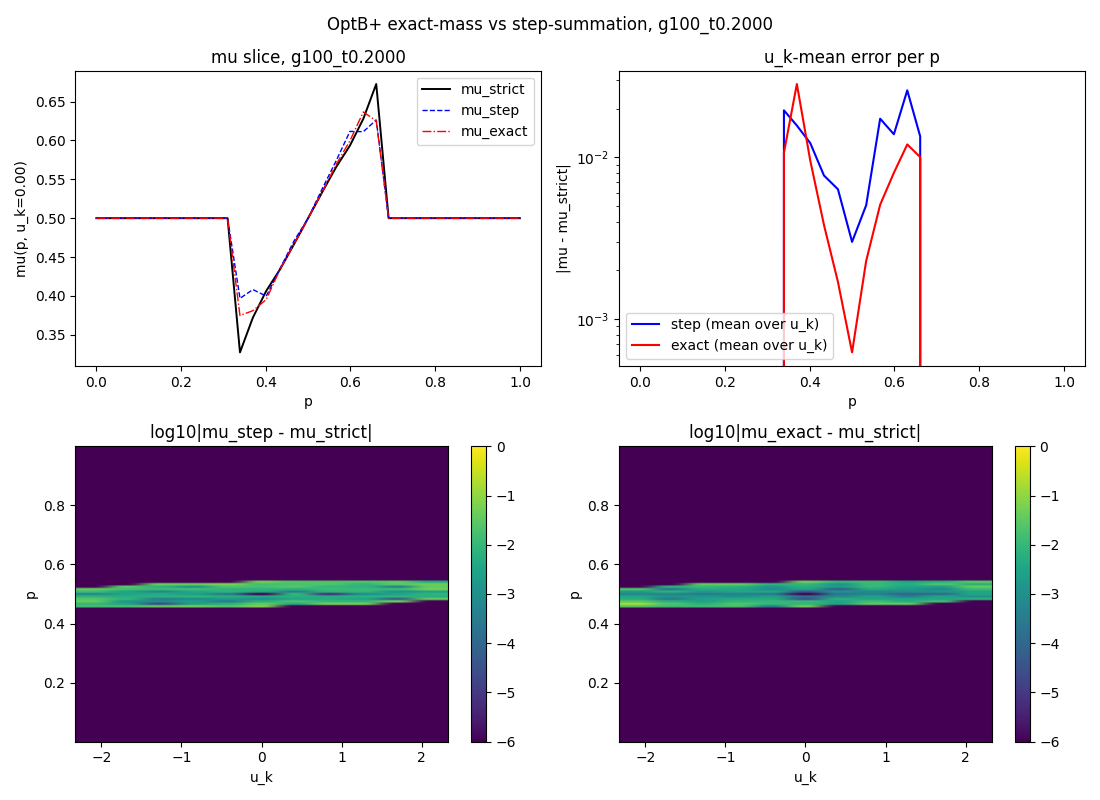
\includegraphics[width=0.49\textwidth]{figs/compare_g100_t0.2000.png}
  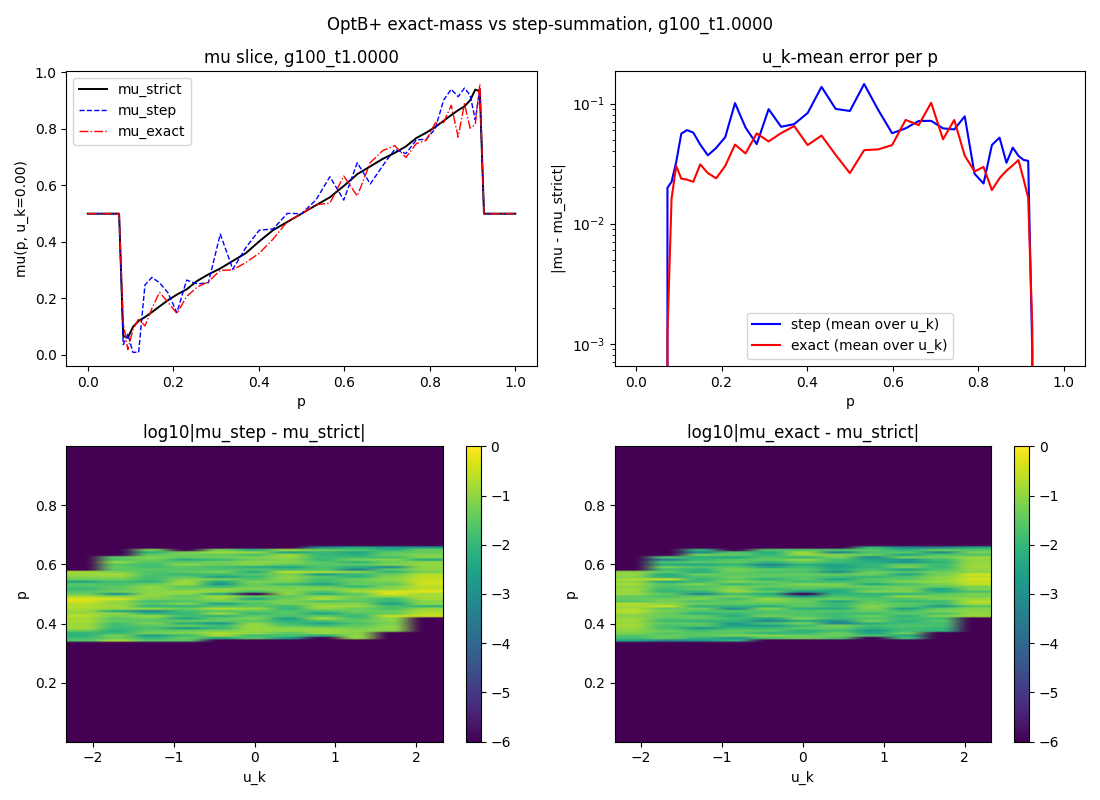
\includegraphics[width=0.49\textwidth]{figs/compare_g100_t1.0000.png}\\[3pt]
  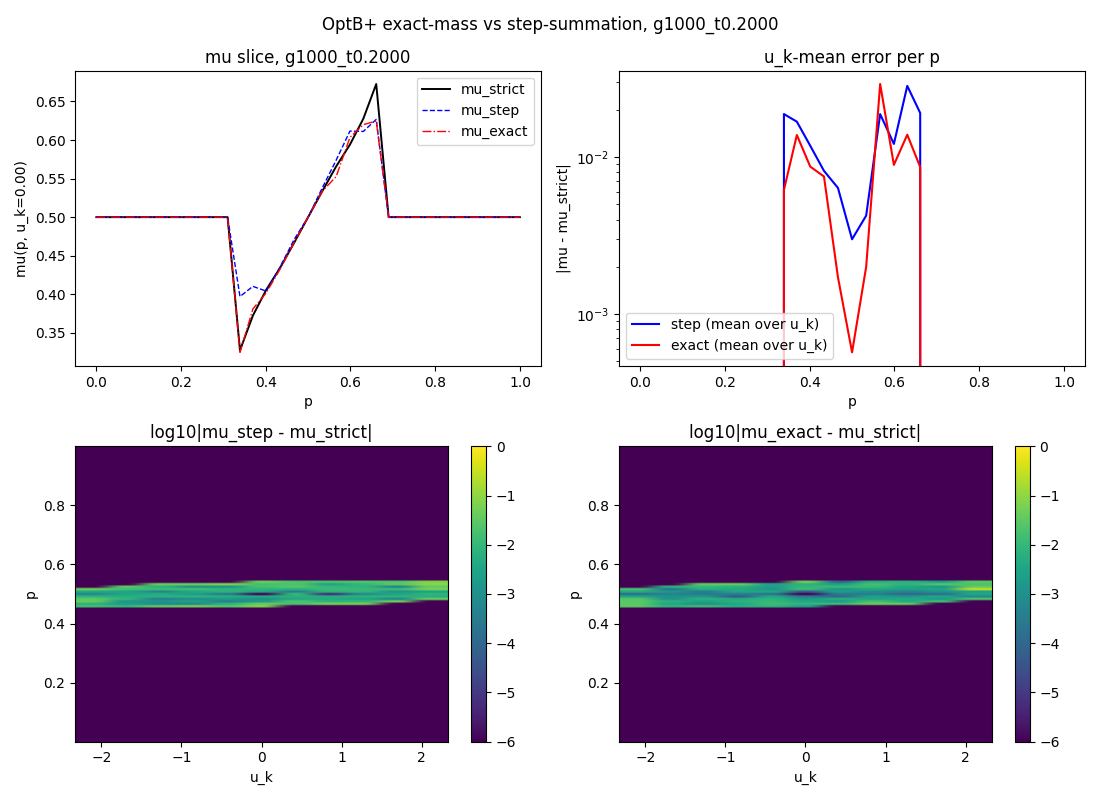
\includegraphics[width=0.49\textwidth]{figs/compare_g1000_t0.2000.png}
  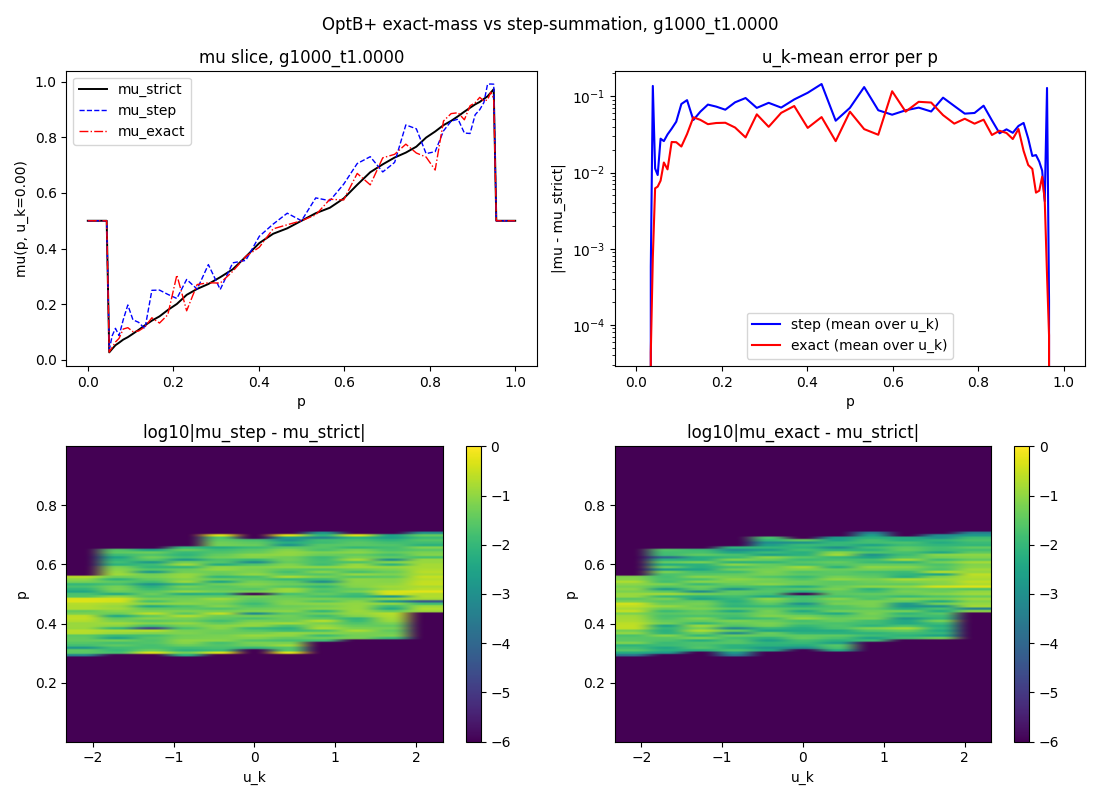
\includegraphics[width=0.49\textwidth]{figs/compare_g1000_t1.0000.png}
  \caption{Step- vs.\ exact-mass $\mu$-tables vs.\ strict-h$=0$.
  Top row: $(\gamma,\tau)=(100,0.2)$ and $(100,1.0)$.
  Bottom row: $(1000,0.2)$ and $(1000,1.0)$.
  The exact-mass density is visibly smoother and tracks the strict
  reference more closely in the interior of $p$-support; both methods
  default to $\mu{=}0.5$ outside the in-support region.}
\end{figure}

\section{Discussion}

\paragraph{What worked.} The exact-mass construction does what was
intended: it distributes each cube cell's Gaussian mass across NQK$^2$
points in $\widehat P$-space, eliminating the within-cell collapse that
biases the step-summation CDF. The median in-support error drops by
$\sim 2\times$ consistently; RMS drops by $\approx 1.5\times$ on the
$\tau{=}1.0$ cells where the support is broad.

\paragraph{What did not improve as hoped.} The max error stays near
$0.4$--$0.5$ in the $\tau{=}1.0$ cells. Inspection shows the worst cells
are at the extreme $p$-grid endpoints where the PCHIP-density of either
sparse-knot or dense-knot empirical CDF oscillates. This is an inherent
limitation of using PCHIP-derivative as the density estimator: the
strict-h$=0$ co-area can resolve $\delta$-spike contributions from
$\nabla P = 0$ points, while a smoothed CDF flattens those.

\paragraph{Cost.} Wall-time per slice goes from $\sim 0.1$ ms (step) to
$\sim 7$ ms (exact, NQK$=8$). For a full $\Phi$ call on the $G=11$ cube,
this raises a single mu-table build from $\approx 0.2$ ms to
$\approx 8$ ms; the cube-clearing pass dominates the overall cost
($\sim 30$ ms), so the impact on $\Phi$ wall-time is moderate ($\sim 2\times$).

\paragraph{Next steps.}
\begin{enumerate}
  \item Implement approach A (closed-form hyperbola decomposition of
        $\{\widehat P\le p\}$) to verify whether the residual is truly
        a PCHIP-floor or a quadrature artifact at the boundary.
  \item Replace PCHIP density by a kernel-band or smoothed-spline
        estimator on the dense micro-cell CDF; this should drop the
        max error materially.
  \item Solve a strict-h$=0$ FP under the exact-mass $\Phi$ to verify
        that the smaller per-step error indeed translates into a closer
        FP $P_{\rm exact}$ vs.\ $P_{\rm strict}$ (bias of the FP, not
        just of the operator at a fixed FP).
\end{enumerate}

\bigskip\noindent\small
Code: \verb|projects/REZN/solver_code/highprec_dd_qd/dd_k3_optB_exact.py|.
Data: \verb|projects/REZN/solved_fixed_points/dd_k3_overnight/optB_exact/|
(\verb|exact_results.json|, per-cell \verb|mu_*.npz|, figures in
\verb|figs/|).

\end{document}
